%Tipo de Documento (articulo, Bemer..etc. )
\documentclass[11pt]{beamer}					% Describe el tipo de documento, y el tamaño de la letra del texto

%BIBLIOTECAS
\usepackage[utf8]{inputenc}					% Define codificación para que permita caracteres latinos (acentos)
\usepackage[spanish,activeacute]{babel} 		% Paquete para poder escribir con tildes y otros caracteres especiales

%\usepackage{amsmath}							% paquete para expresiones matemáticas
%\usepackage{amsfonts}						% paquete para escritura de ecuaciones 
%\usepackage{amssymb}							% paquete para caracteres especiales para ecuaciones 

\usepackage{svg}								% Se utiliza para incluir imágenes vectorizadas en el documento (.pdf)
\usepackage{hyperref}						% Para hipervinculos

\usepackage{lmodern}							% http://ctan.org/pkg/lm
\usepackage{listings}						% Para el código fuente
\usepackage{xcolor}							% Para el color en código fuente
\usepackage{graphicx}						% Para incluir imágenes
\graphicspath{{Imagenes/}}					% Directorio de imágenes

\bibliographystyle{apalike} 					% Bibliografia tipo APA

\definecolor{limegreen}{RGB}{50,100,50}		% Definición de color
\definecolor{azul}{RGB}{120,120,210}
\lstdefinestyle{base}{						% Para el color en código fuente
	language=C,
	emptylines=1,
	breaklines=true,
	showspaces=false,
	showstringspaces=false,
	extendedchars=true,
	basicstyle=\ttfamily\color{black},
	moredelim=**[is][\color{limegreen}]{'}{'},
	moredelim=**[is][\color{blue}]{&}{&},
}				
%\lstset{numbers=left, numberstyle=\tiny, stepnumber=1, numbersep=5pt}	% Muestra numeración al lado del código


%PRESENTACIÓN
\mode<presentation>
{
    %Tema de la presentación 	
	\usetheme{Frankfurt}
    %Color del Tema de la presentación 	
	\usecolortheme{orchid}
}

%Inicio del documento 
\begin{document}
	
		% Titulo Corto y Completo de La presentación.
		\title[Titulo Corto]{Tricks and Solutions}
		%Logo Gráfica Escudo Universidad Vectorizado.
		\logo{
\includegraphics[scale=0.08]{escudoud}}
		%Autor, Universidad, Fecha..
		\author{Yeny Katherine Muñoz Nuñez}
		\institute[UD]{Universidad Distrital Francisco José de Caldas}
		\date{\today}

% Diapositiva 1
     	%Iniciar Diapositiva
		\begin{frame}
	       	%Titulo de la pagina
			\titlepage 
		\end{frame}
	
% Diapositiva 2
     	%Iniciar Diapositiva
     	\begin{frame}
        %Titulo de la diapositiva
		\frametitle{Indice}	
	    %Tabla de contenido	
		\tableofcontents
		\end{frame}
	
% Título Primera Sección
\section{Chunk Options}
	
	\subsection{Option Aliases}
		\begin{frame}
		    	%Titulo Diapositiva.	
			\frametitle{Chunk Options - Option Aliases}
				%Titulo Bloque 1				
				\begin{block}{En el inicio de un documento:}
					\begin{small}
						\begin{center}
						
\includegraphics[scale=1]{Aliases1} 
						\end{center}
					\end{small}
				\end{block}
				\begin{block}{Se puede hacer uso de 'w' y 'h' :}
					\begin{small}
						\begin{center}
						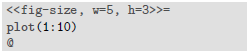
\includegraphics[scale=1]{Aliases2} 
						\end{center}
					\end{small}
				\end{block}
				\begin{block}{Lo anterior es equivalente a:}
					\begin{small}
						\begin{center}
						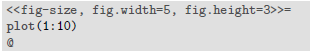
\includegraphics[scale=1]{Aliases3} 
						\end{center}
					\end{small}
				\end{block}
		\end{frame}
	\subsection{Option Templates}
		\begin{frame}
		    	%Titulo Diapositiva.	
			\frametitle{Chunk Options - Option Templates}
				%Titulo Bloque 1				
				\begin{block}{Una plantilla es un conjunto de opciones:}
					\begin{small}
						\begin{center}
						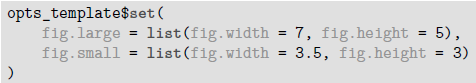
\includegraphics[scale=0.8]{Templates1} 
						\end{center}
					\end{small}
				\end{block}
				\begin{block}{Después de creada la plantilla, podemos simplemente usar el nombre asignado:}
					\begin{small}
						\begin{center}
						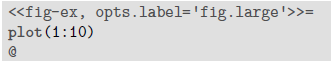
\includegraphics[scale=0.8]{Templates2} 
						\end{center}
					\end{small}
				\end{block}
				\begin{block}{Lo anterior es equivalente a:}
					\begin{small}
						\begin{center}
						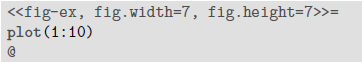
\includegraphics[scale=0.7]{Templates3} 
						\end{center}
					\end{small}
				\end{block}
		\end{frame}
	\subsection{Code in Appendix}
		\begin{frame}
		    	%Titulo Diapositiva.	
			\frametitle{Chunk Options - Code in Appendix}
				%Titulo Bloque 1				
				\begin{block}{A veces no queremos mostrar los trozos de código en el cuerpo del informe:}
					\begin{small}
						\begin{center}
						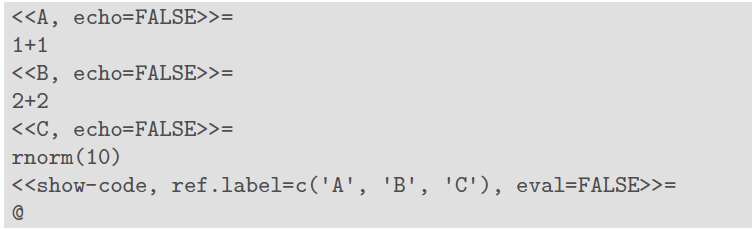
\includegraphics[scale=0.5]{Appendix1} 
						\end{center}
					\end{small}
				\end{block}
				\begin{block}{Si se tienen muchos chunks en un documento, se puede hacer uso de:}
					\begin{small}
						\begin{center}
						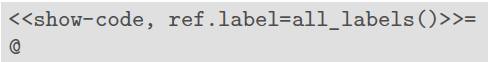
\includegraphics[scale=0.6]{Appendix2} 
						\end{center}
					\end{small}
				\end{block}
		\end{frame}
	\subsection{Local R Options}
		\begin{frame}
		    	%Titulo Diapositiva.	
			\frametitle{Chunk Options - Local R Options}
				%Titulo Bloque 1				
				\begin{block}{R.options permite tomra una lista de R por un código chunk:}
					\begin{small}
						\begin{center}
						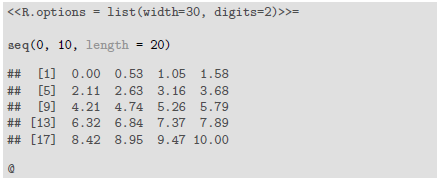
\includegraphics[scale=0.9]{Options1} 
						\end{center}
					\end{small}
				\end{block}
		\end{frame}
		
\section{Package Options}

		\begin{frame}
		    	%Titulo Diapositiva.	
			\frametitle{Package Options}
				%Titulo Bloque 1				
				\begin{block}{Para ver más información respecto a los chuck en un código fuente, se puede activar el modo detallado por medio del comando:}
						\begin{center}
						
\includegraphics[scale=0.9]{Package1} 
						\end{center}
				\end{block}
				\begin{block}{root.dir se puede utilizar para establecer el directorio de trabajo en el código chunk:}
					\begin{small}
						\begin{center}
						
\includegraphics[scale=0.9]{Package2} 
						\end{center}
					\end{small}
				\end{block}
				\begin{block}{Para los chuck que no están etiquetados:}
					\begin{small}
						\begin{center}
						
\includegraphics[scale=0.9]{Package3} 
						\end{center}
					\end{small}
				\end{block}
		\end{frame}

\section{Typesetting}

	\subsection{Output Width}
		\begin{frame}
		    	%Titulo Diapositiva.	
			\frametitle{Typesetting - Output Width}
				%Titulo Bloque 1				
				\begin{block}{Cuando vemos que el código fuente o la salida de texto es demasiado amplia, podemos utilizar una opción de menor anchura:}
						\begin{center}
						
\includegraphics[scale=0.85]{Width1} 
						\end{center}
				\end{block}
				\begin{block}{Sin embargo, existen casos donde la cadena de caracteres es demasiado larga en el código fuente:}
					\begin{small}
						\begin{center}
						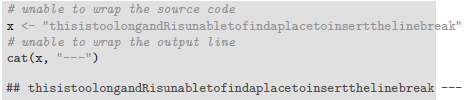
\includegraphics[scale=0.6]{Width2} 
						\end{center}
					\end{small}
				\end{block}
				\begin{block}{Es posible dividirla en pedazos más pequeños de forma manual y unirla nuevamente como se muestra a continuación:}
					\begin{small}
						\begin{center}
						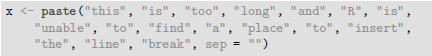
\includegraphics[scale=0.6]{Width3} 
						\end{center}
					\end{small}
				\end{block}
		\end{frame}
	\subsection{Box Padding}
		\begin{frame}
		    	%Titulo Diapositiva.	
			\frametitle{Typesetting - Box Padding}
				%Titulo Bloque 1				
				\begin{block}{Si sentimos que el relleno por defecto de la caja es demasiado ajustado, se puede restablecer la longitud:}
						\begin{center}
						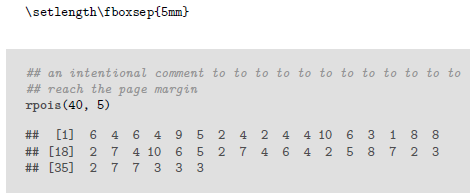
\includegraphics[scale=0.8]{Padding1} 
						\end{center}
				\end{block}
				\begin{block}{Se puede definir la misma clase en CSS de la siguiente forma:}
					\begin{small}
						\begin{center}
						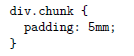
\includegraphics[scale=0.7]{Padding2} 
						\end{center}
					\end{small}
				\end{block}
		\end{frame}
	\subsection{Beamer}
		\begin{frame}
		    	%Titulo Diapositiva.	
			\frametitle{Typesetting - Beamer}
				%Titulo Bloque 1				
				\begin{block}{Ejemplo de uso de knitr en diapositiva beamer:}
						\begin{center}
						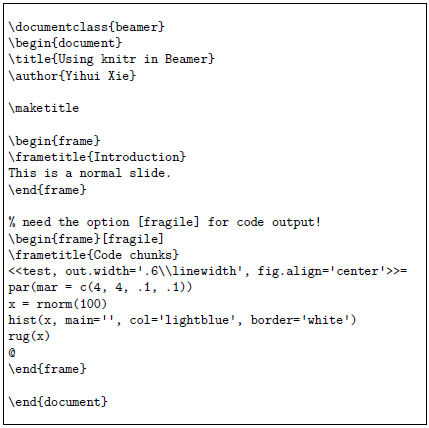
\includegraphics[scale=0.6]{Beamer1} 
						\end{center}
				\end{block}
		\end{frame}
		\begin{frame}
		    	%Titulo Diapositiva.	
			\frametitle{Typesetting - Beamer}
				\begin{block}{Ejemplo de diapositiva con beamer:}
					\begin{small}
						\begin{center}
						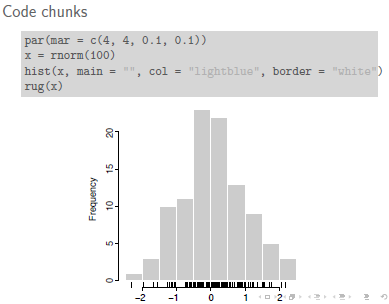
\includegraphics[scale=0.7]{Beamer2} 
						\end{center}
					\end{small}
				\end{block}
		\end{frame}
	\subsection{Suppress Long Output}
		\begin{frame}
		    	%Titulo Diapositiva.	
			\frametitle{Typesetting - Suppress Long Output}
				%Titulo Bloque 1				
				\begin{block}{Omitir partes del libro, debido a que los resultados son muy largos:}
						\begin{center}
						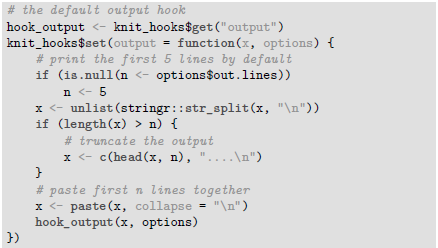
\includegraphics[scale=0.5]{Suppress1} 
						\end{center}
				\end{block}
				\begin{block}{La idea básica de que la regla definida anteriormente es:}
					\begin{small}
						\begin{center}
						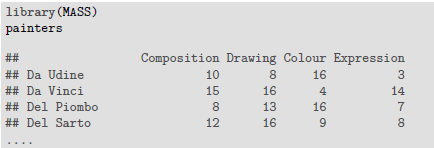
\includegraphics[scale=0.5]{Suppress2} 
						\end{center}
					\end{small}
				\end{block}
		\end{frame}

\section{Utilities}
	\subsection{R Package Citation}
		\begin{frame}
		    	%Titulo Diapositiva.	
			\frametitle{Utilities - R Package Citation}
				%Titulo Bloque 1				
				\begin{block}{Por defecto se recoge los paquetes cargados en la sesión actual de R y extrae su información de la cita:}
						\begin{center}
						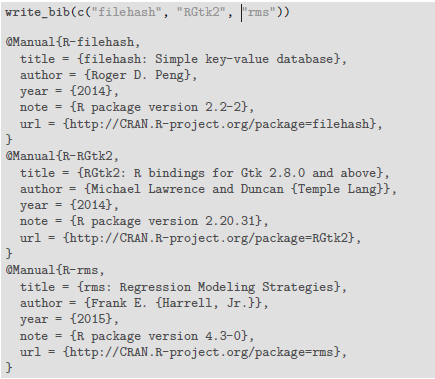
\includegraphics[scale=0.4]{Citation} 
						\end{center}
				\end{block}
				\begin{block}{Si el archivo principal el chunk se escribe de la siguiente forma:}
					\begin{small}
						\begin{center}
						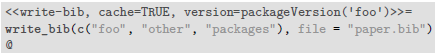
\includegraphics[scale=0.5]{Citation2} 
						\end{center}
					\end{small}
				\end{block}
		\end{frame}

\section{Debugging}
		\begin{frame}
		    	%Titulo Diapositiva.	
			\frametitle{Debugging}
				%Titulo Bloque 1				
				\begin{block}{Debugging}
Cuando se produce un error que no se observa claramente en la pantalla, podemos utilizar herramientas de depuración comunes, tales como traceback () (para ver el paso a paso que ha conducido al error), debug () o browser ().
				\end{block}
		\end{frame}

\section{Multilingual Support}
		\begin{frame}
		    	%Titulo Diapositiva.	
			\frametitle{Multilingual Support}
				%Titulo Bloque 1				
				\begin{block}{Si el documento de origen no se ha codificado con la codificación nativa del sistema actual, tendremos que especificar manualmente su codificación mediante el argumento de codificación en:}
						\begin{center}
						
\includegraphics[scale=1]{Support} 
						\end{center}
				\end{block}
		\end{frame}

%BIBLIOGRAFIA
\section{Bibliografía}
  	\begin{frame}
  		%Titulo de la diapositiva
 		\frametitle{Bibliografía}
  			%Para que aparezca toda la bibliografia que citamos en el documento.	
\begin{thebibliography}{}

\bibitem[Yihui Xie, 2013]{Biblio1}
Yihui Xie (2013).
\newblock {\em Dynamic Documents with R and knitr}.
\newblock CRC Press 2016. 2 Ed.

\end{thebibliography}

       	\end{frame}

\end{document}